% !TeX spellcheck = en_US
\section{Problem 10}

\subsection{Question A}

The patterns that we want to separate are plotted in figure~\ref{fig:prob_10_patterns}.

\begin{figure}[H]
	\centering
	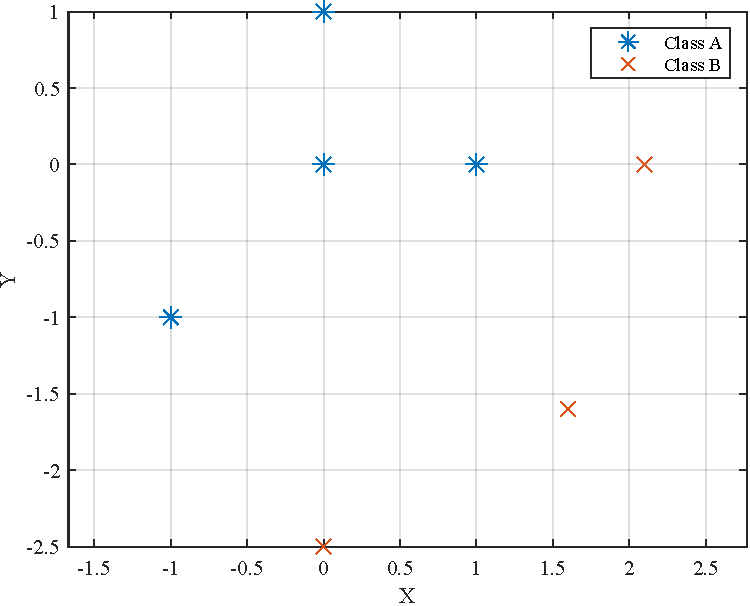
\includegraphics[width=0.5\textwidth]{../Problem 10/patterns.pdf}
	\caption{Plot of patterns}
	\label{fig:prob_10_patterns}
\end{figure}

We can clearly see that there can be a straight line that can separate the two classes, thus an ADALINE neural network can work in classification for this system.

\subsection{Question B}

The designed ADALINE neural network will be of the following architecture
\begin{itemize}
	\item Input Layer: Since the patterns are two-dimensional (each pattern has two values), the input layer will have two nodes.
	\item Output Layer: The output layer will have one node. This is because the task is a binary classification. The output node will use a linear activation function, as is standard in ADALINE networks.
	\item Weights and Bias: There will be two weights (one for each input node) and one bias. The weights and bias are parameters that the network will learn during the training process.
	\item Learning Rule: The network will use the LMS learning rule (\textit{Least Mean Square}) to update the weights and bias. This rule minimizes the mean square error between the network's output and the target output.
\end{itemize}

This architecture described beforehand is shown in figure~\ref{fig:prob10_adaline_architecture}.
\begin{figure}[htpb]
	\centering
	\includesvg[width=0.7\textwidth]{../Problem 10/prob10_adaline.svg}
	\caption{ADALINE neural network architecture}
	\label{fig:prob10_adaline_architecture}
\end{figure}

\subsection{Question c}
%The ADALINE neural network created can be described from the following MATLAB code in listing~\ref{listing:prob10_matlab_code}. So, in order to display the final weights, we can run the algorithm and let it calculate the final wights.
The ADALINE neural network mentioned above was coded in MATLAB. During training, we plotted its weights and bias in order to check their progression. Maximum iteration value was defined in code to be $10^4$ and minimum error to end train and consider the solutions converged is $epsilon$ of the machine, specifically $eps = 2.2204\ 10^{-16}$.

After converging, the final weights and bias are presented in table~\ref{table:prob10_final_weight_bias} below. 

\begin{figure}[htpb]
	\centering
	\begin{subfigure}[l]{0.47\textwidth}
		\centering
		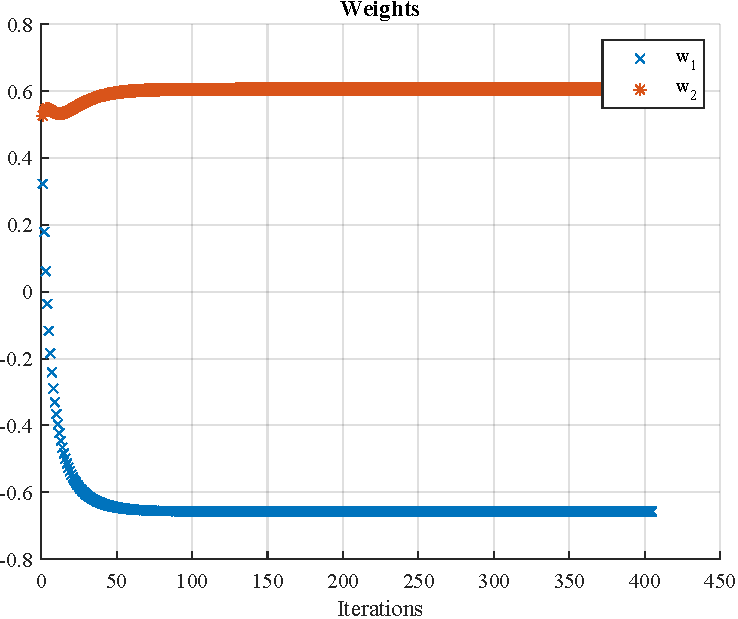
\includegraphics[width=\textwidth]{../Problem 10/prob10_adaline_weights.pdf}
	\end{subfigure}
	\hspace{1mm}
	\begin{subfigure}[r]{0.47\textwidth}
		\centering
		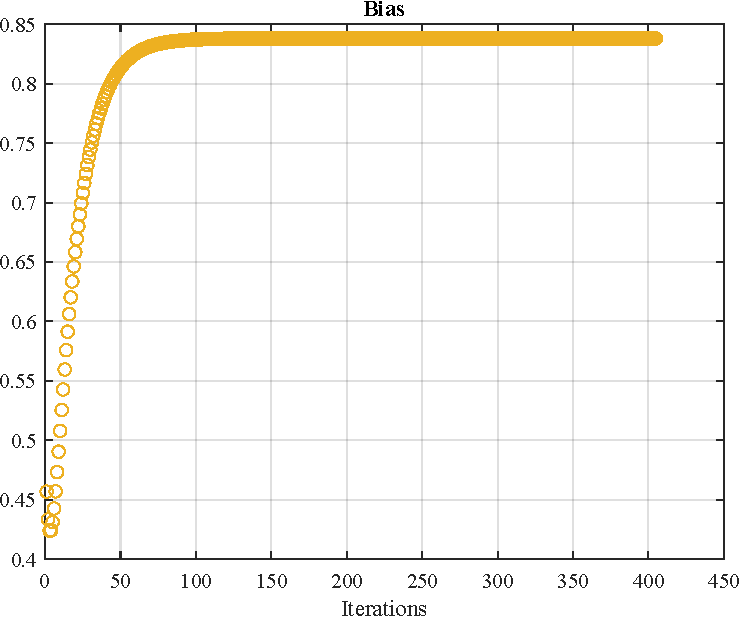
\includegraphics[width=\textwidth]{../Problem 10/prob10_adaline_biases.pdf}
	\end{subfigure}
	\caption{Plots of weights and biases during training}
	\label{fig:prob10_plot_weights_biases}
\end{figure}

\begin{table}[H]
	\centering
	\begin{tblr}{hlines, vlines, colspec={ccc}}
		\textbf{Weight 1} & \textbf{Weight 2} & \textbf{Bias} \\
		-0.6564 & 0.6052 & 0.8407 \\
	\end{tblr}
	\caption{Final table of weights and bias}
	\label{table:prob10_final_weight_bias}
\end{table}